\chapter{Tóm tắt lý thuyết}
\section{Mô hình động học phân tử và sự chuyển thể}
\subsection{Mô hình động học phân tử}
\begin{itemize}
	\item Vật chất được cấu tạo từ các hạt riêng biệt gọi là phân tử.
	\item Các phân tử chuyển động hỗn loạn không ngừng, gọi là chuyển động nhiệt. Nhiệt độ càng cao thì tốc độ trung bình của các phân tử càng lớn.
	\item Giữa các phân tử có lực liên kết phân tử (hút và đẩy).
\end{itemize}
\subsection{Cấu trúc của vật chất}
\begin{center}
	\begin{tabular}{|L{4cm}|L{4cm}|L{4cm}|L{4cm}|}
		\hline
		\thead{Cấu trúc}&\thead{Thể khí}& \thead{Thể rắn}&\thead{Thể lỏng}\\
		\hline
		Khoảng cách giữa các phân tử & Rất xa nhau (gấp hàng chục lần kích thước phân tử) & Rất gần nhau (cỡ kích thước phân tử) & Xa nhau\\
		\hline
		Sự sắp xếp của các phân tử & 	Không có trật tự & Trật tự & Kém trật tự hơn thể rắn\\
		\hline
		Chuyển động của các phân tử & Chuyển động hỗn loạn & Chỉ dao động quanh vị trí cân bằng cố định & Dao động quanh vị trí cân bằng luôn thay đổi\\
		\hline
		Minh họa chuyển động của các phân tử & \begin{center}
			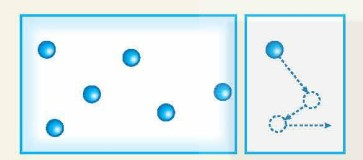
\includegraphics[width=0.8\linewidth]{../figs/G12C1-1}
		\end{center}&\begin{center}
		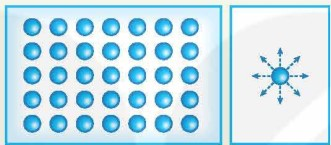
\includegraphics[width=0.8\linewidth]{../figs/G12C1-2}
		\end{center}(Chất rắn kết tinh) &\begin{center}
		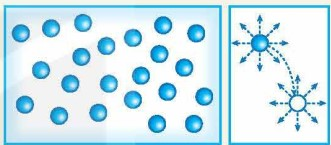
\includegraphics[width=0.8\linewidth]{../figs/G12C1-3}
		\end{center}\\
		\hline
	\end{tabular}
\end{center}
\subsection{Các quá trình chuyển thể}
\begin{itemize}
	\item Các chất có thể chuyển từ thể này sang thể khác.
	\item Cấu trúc của chất thay đổi khi chuyển thể.
\end{itemize}
\begin{center}
	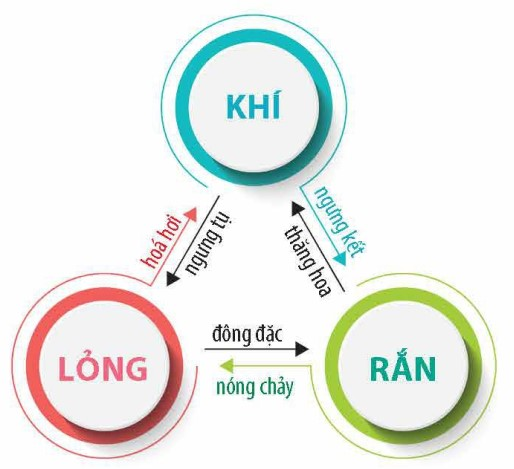
\includegraphics[width=0.35\linewidth]{../figs/G12C1-4}
\end{center}
\luuy{Sự hóa hơi thể hiện qua hai hình thức: sự bay hơi và sự sôi
\begin{itemize}
	\item Sự bay hơi là sự hóa hơi xảy ra trên bề mặt chất lỏng. Sự bay hơi xảy ra ở bất kì nhiệt độ nào.
	\item Sự sôi là sự hóa hơi xảy ra ở bên trong và trên bề mặt chất lỏng. Sự sôi xảy ra ở nhiệt độ sôi.
	\end{itemize}}
\section{Nội năng - Định luật I nhiệt động lực học}
\subsection{Nội năng}
\begin{itemize}
	\item Nội năng của một vật là tổng động năng và thế năng tương tác của các phân tử cấu tạo nên vật.
	\item Nội năng được kí hiệu là $U$ và có đơn vị là $\si{\joule}$.
	\item Nội năng của vật phụ thuộc vào nhiệt độ $T$ và thể tích $V$ của vật.
	\item Có thể làm thay đổi nội năng của vật bằng cách: thực hiện công, truyền nhiệt.
\end{itemize}
\subsection{Định luật I nhiệt động lực học}
Độ biến thiên nội năng của vật bằng tổng công và nhiệt lượng mà vật nhận được.
\begin{equation}
	\Delta U=Q+A
\end{equation}
\begin{center}
	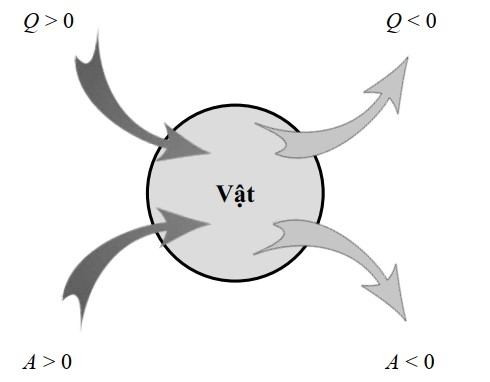
\includegraphics[width=0.3\linewidth]{../figs/G12C1-5}
\end{center}
\section{Thang nhiệt độ}
\subsection{Chiều truyền năng lượng nhiệt giữa hai vật chênh lệch nhiệt độ tiếp xúc nhau}
\begin{itemize}
	\item Khi hai vật chênh lệch nhiệt độ tiếp xúc nhau, năng lượng nhiệt luôn truyền từ vật có nhiệt độ cao hơn sang vật có nhiệt độ thấp hơn.
	\item Quá trình truyền nhiệt kết thúc khi hai vật ở cùng một nhiệt độ (cân bằng nhiệt với nhau).
\end{itemize}
\subsection{Các thang nhiệt độ}
\begin{itemize}
	\item \textit{Thang nhiệt độ Celsius}: Nhiệt độ đóng băng của nước tinh khiết là $\SI{0}{\celsius}$ và nhiệt độ sôi của nước tinh khiết là $\SI{100}{\celsius}$ ở áp suất tiêu chuẩn. Nhiệt độ trong thang Celsius thường được kí hiệu là $t$.
	\item \textit{Thang nhiệt độ Kelvin}: Nhiệt độ thấp nhất mà các vật có thể có được là $\SI{0}{\kelvin}$ (độ không tuyệt đối) và nhiệt độ mà nước tinh khiết có thể tồn tại đồng thời ở cả ba thể rắn, lỏng và hơi là $\SI{273.16}{\kelvin}$. Nhiệt độ trong thang Kelvin thường được kí hiệu là $T$.
	\begin{equation}
		\xsi{T}{\left(\si{\kelvin}\right)}=\xsi{t}{\left(\si{\celsius}\right)}+273
	\end{equation}
	
\end{itemize}
\manatip{Công thức chuyển đổi thang nhiệt độ $X$ sang thang nhiệt độ $Z$ có nhiệt độ đóng băng và nhiệt độ sôi  của nước tinh khiết lần lượt là $\left(X_b,X_s\right)$, $\left(Z_b, Z_s\right)$ trong trường hợp 2 thang nhiệt độ quan hệ tuyến tính với nhau:
	\begin{equation}
		\dfrac{X-X_b}{X_s-X_b}=\dfrac{Y-Y_b}{Y_s-Y_b}
	\end{equation}
	
}
\subsection{Nhiệt độ không tuyệt đối}
Nhiệt độ không tuyệt đối $\left(\SI{0}{\kelvin}\right)$ là nhiệt độ mà tại đó tất cả các chất có động năng chuyển động nhiệt của các phân tử hoặc nguyên tử bằng không và thế năng của chúng là tối thiểu.
\section{Nhiệt dung riêng, nhiệt nóng chảy riêng, nhiệt hóa hơi riêng}
\subsection{Nhiệt dung riêng}
\begin{itemize}
	\item Nhiệt dung riêng của một chất có giá trị bằng nhiệt lượng cần cung cấp để làm tăng nhiệt độ của $\SI{1}{\kilogram}$ chất đó lên $\SI{1}{\kelvin}$.
	\begin{equation}
		c=\dfrac{Q}{m\left(T_2-T_1\right)}
	\end{equation}
	\item Trong hệ SI, đơn vị đo nhiệt dung riêng là $\si{\joule/\left(\kilogram\cdot\kelvin\right)}$.
\end{itemize}
Nhiệt lượng mà một vật có khối lượng $m$ trao đổi khi thay đổi nhiệt độ từ $T_1$ đến $T_2$ được xác định bởi biểu thức: $Q = mc\left(T_2 – T_1\right)$\\
Trong hệ SI, đơn vị đo nhiệt lượng là $\si{\joule}$. Ngoài ra, nhiệt lượng còn được đo bằng đơn vị $\si{cal}$
$$\SI{1}{cal}=\SI{4,186}{\joule}.$$
\subsection{Nhiệt nóng chảy riêng}
\begin{itemize}
	\item Nhiệt nóng chảy riêng của một chất có giá trị bằng nhiệt lượng cần cung cấp cho $\SI{1}{\kilogram}$ chất đó chuyển hoàn toàn từ thể rắn sang thể lỏng tại nhiệt độ nóng chảy.\\
	\begin{equation}
		\lambda=\dfrac{Q}{m}
	\end{equation}
	\item Trong hệ SI, đơn vị đo nhiệt nóng chảy riêng là $\si{\joule/\kilo}$.
\end{itemize}
\subsection{Nhiệt hóa hơi riêng}
\begin{itemize}
	\item Nhiệt hoá hơi riêng của một chất lỏng có giá trị bằng nhiệt lượng cần cung cấp cho $\SI{1}{\kilogram}$ chất lỏng đó hoá hơi hoàn toàn ở nhiệt độ sôi.
	\begin{equation}
		L=\dfrac{Q}{m}
	\end{equation}
	\item Trong hệ SI, đơn vị đo nhiệt hoá hơi riêng là $\si{\joule/\kilogram}$.
\end{itemize}
